\documentclass[11pt,letterpaper]{article}

%%%%%%%%%%%%%%%%%%%%%%%%%%%%%%%%%%%
% IMPORTACIÓN DE CONFIGURACIONES
%%%%%%%%%%%%%%%%%%%%%%%%%%%%%%%%%%%

\input{configuracion}

%%%%%%%%%%%%%%%%%%%%%%%%%%%%
% INICIO DE DOCUMENTO
%%%%%%%%%%%%%%%%%%%%%%%%%%%%

\begin{document}

%%%%%%%%%%%%%%%%%%%%%%%%%%%%
% ENCABEZADO
%%%%%%%%%%%%%%%%%%%%%%%%%%%%
\begin{center}
    \begin{minipage}{3cm}
    	\begin{center}
    		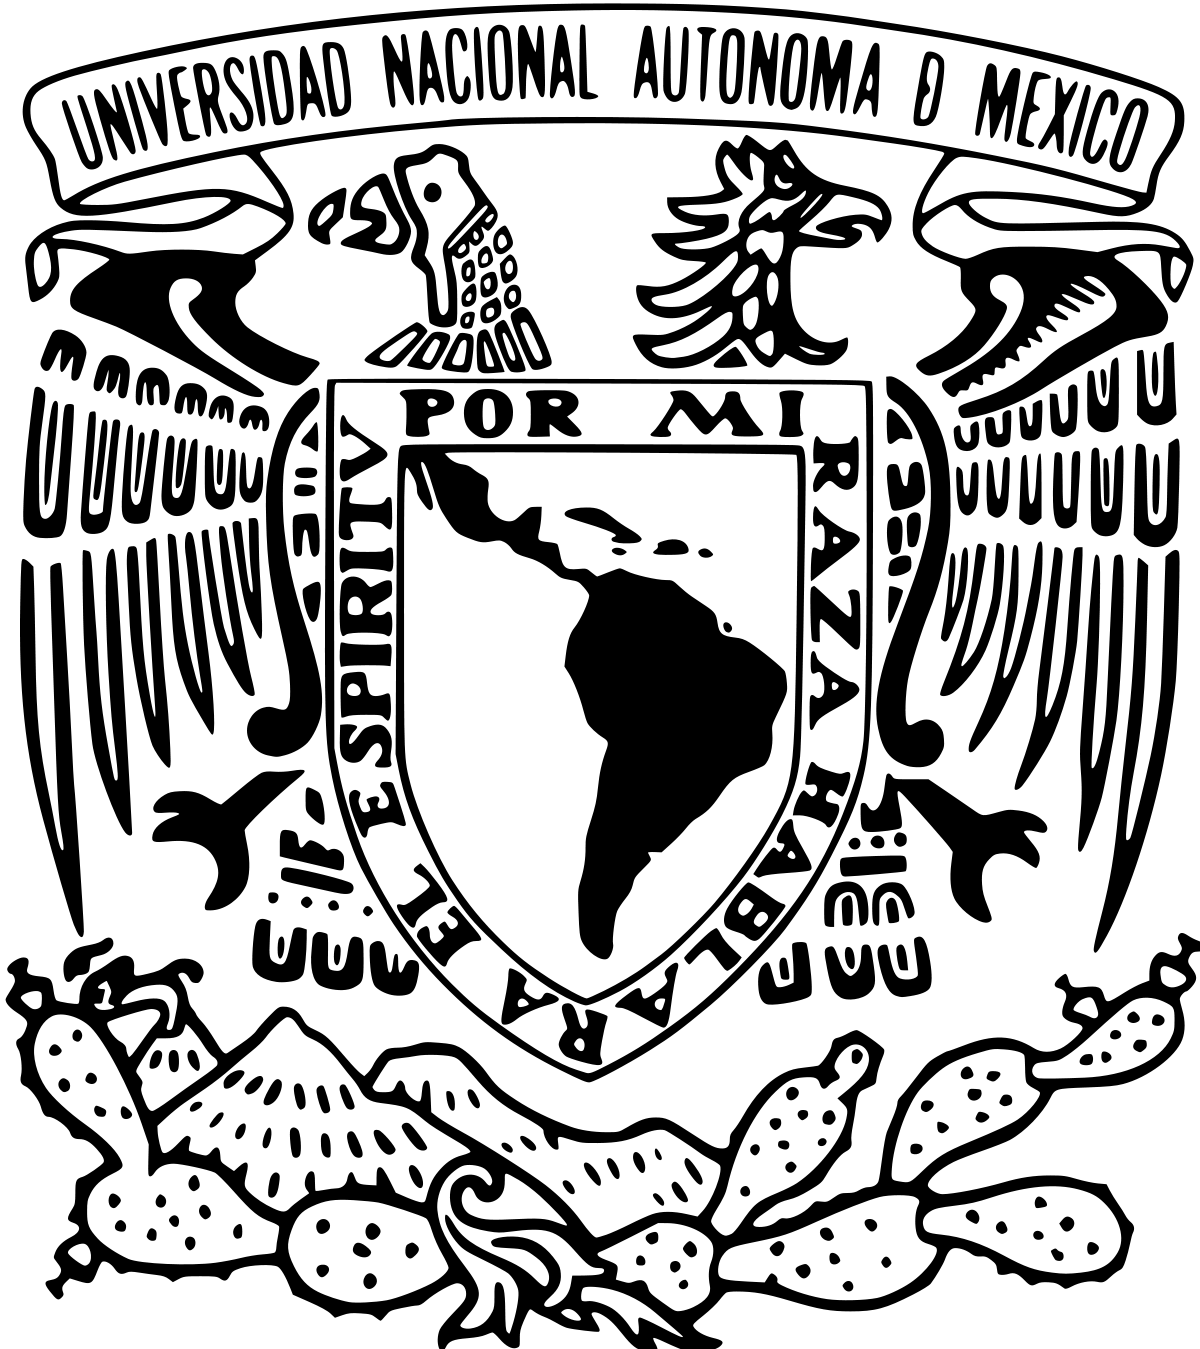
\includegraphics[height=3.4cm]{Logo_UNAM.png}
    	\end{center}
    \end{minipage}\hfill
    \begin{minipage}{10cm}
    	\begin{center}
    	\textbf{\large Universidad Nacional Autónoma de México}\\[0.1cm]
        \textbf{Facultad de Ciencias}\\[0.1cm]
        \textbf{Geometría Analítica $|$ Grupo 4025}\\[0.1cm]
        Tarea 1 - Ejercicios del Bracho\\[0.1cm]
        Jorge Ivan Ramos Cuenca\\[0.1cm]
        \today
    	\end{center}
    \end{minipage}\hfill
    \begin{minipage}{3cm}
    	\begin{center}
    		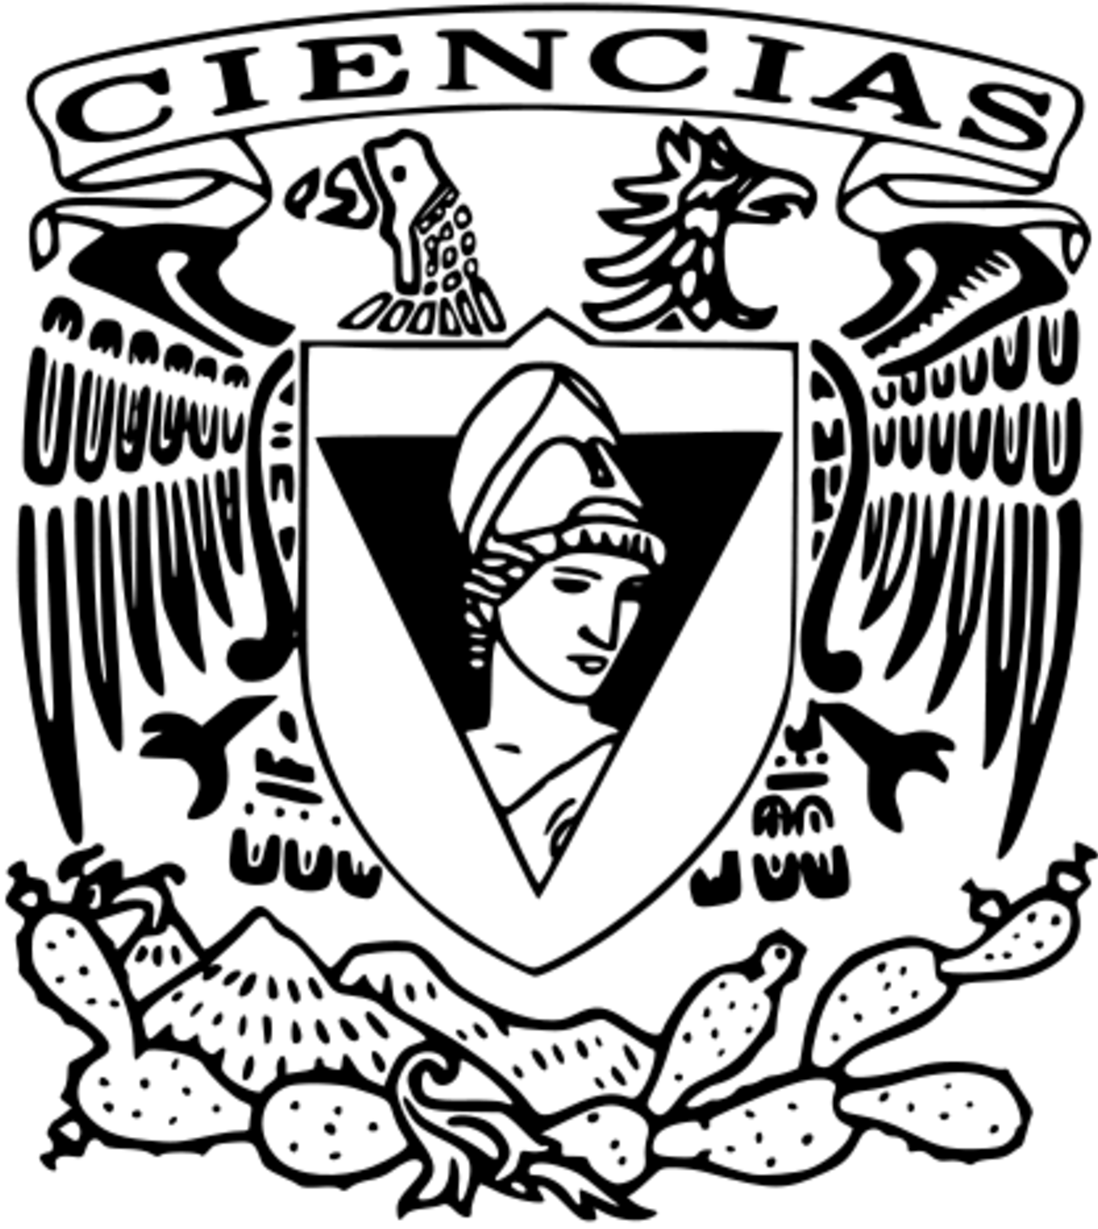
\includegraphics[height=3.4cm]{Logo_FC.png}
    	\end{center}
    \end{minipage}
\end{center}

\rule{17cm}{0.1mm}

%%%%%%%%%%%%%%%%%%%%%%%%%%%%
% FIN DE ENCABEZADO
%%%%%%%%%%%%%%%%%%%%%%%%%%%%

\begin{intro}
    Realizar los siguientes ejercicios
\end{intro}

\begin{inciso}{Ejercico 1.17}
- Demuestra que si \( x \in \mathbb{R}^n \) es distinto de \( 0 \), y \( t, s \in \mathbb{R} \) son tales que \( tx = sx \), entonces \( t = s \). (Es decir, si \( x \neq 0 \) está permitido ''cancelarlo'' aunque sea vector.)

\begin{demostracion}{}
- Partimos de la igualdad dada: 
\begin{equation*}
    tx=sx
\end{equation*}
Luego, restamos $sx$ en ambos lados quedando: 
\begin{equation*}
    tx - sx = 0
\end{equation*}
Ahora bien, podemos factorizar: 
\begin{equation*}
    (t-s)x=0
\end{equation*}
Dado que $x \neq 0$, al menos una de sus componentes es no nula. Supongamos que la componente $x_i \neq 0$, la única posibilidad es que el escalar $t-s$ sea cero: 
\begin{equation*}
    t-s=0 \quad \Rightarrow \quad t=s
\end{equation*}

\fbox{$\therefore$ Si \( x \in \mathbb{R}^n \) es distinto de \( 0 \), y \( t, s \in \mathbb{R} \) son tales que \( tx = sx \), entonces \( t = s \)}

\end{demostracion}
\end{inciso}

\begin{inciso}{Ejercico 1.24}
- Dados dos vectores \( \mathbf{u} \) y \( \mathbf{v} \) en \( \mathbb{R}^n \), el \textit{paralelogramo} que definen tiene como vértices los puntos \( \mathbf{0} \), \( \mathbf{u} \), \( \mathbf{v} \) y \( \mathbf{u} + \mathbf{v} \) (como en la figura). Demuestra que sus \textit{diagonales}, es decir, los segmentos de \( \mathbf{0} \) a \( \mathbf{u} + \mathbf{v} \) y de \( \mathbf{u} \) a \( \mathbf{v} \) se intersectan en su punto medio.

\begin{demostracion}{}
- Para éste problema, podemos parametrizar tanto la diagonal que va de $0 \text{ a } u+v$ como la diagonal que va de $u \text{ a } v$:

\begin{itemize}
    \item Todo punto en la diagonal de $0 \text{ a } u+v$ se puede escribir como: 
    \begin{equation*}
        p(t)= t(u+v), \quad \text{donde } t\in [0,1].
    \end{equation*}
    En particular, cuando $t=1/2$, obtenemos
    \begin{equation*}
        p \left(\frac{1}{2}\right) = \frac{1}{2}(u+v),
    \end{equation*}
    que es claramente el punto medio entre $0 \text{ y } u+v$.
    \item Todo punto en la diagonal de $u \text{ a } v$ se puede expresar como 
    \begin{equation*}
        q(s)=(1-s)u + sv, \quad \text{donde } s \in [0,1].
    \end{equation*}
    Para $s=\frac{1}{2}$ obtenemos: 
    \begin{equation*}
        q\left(\frac{1}{2}\right)= \frac{1}{2}u + \frac{1}{2} v = \frac{1}{2}(u+v),
    \end{equation*}
    que es el punto medio entre $u \text{ y } v$. 
    Como conclusión, se nos muestra en ambas parametrizaciones que el punto $\frac{1}{2} (u + v)$ pertenece a ambas diagonales. Por lo tanto, las diagonales del paralelogramo se intersectan en su punto medio. 
\end{itemize}
\end{demostracion}
\end{inciso}

\begin{inciso}{Ejercicio 1.26}
- Sean $a, \, b \text{ y } c$ tres puntos distintos entre sí. Demuestra que si $a$ está en la recta que pasa por $b \text{ y } c$, entonces $b$ está en la recta que pasa por $a \text{ y }c$.

\begin{demostracion}{}
- Dado que \( a, b \) y \( c \) son tres puntos distintos y se nos dice que \( a \) está en la recta que pasa por \( b \) y \( c \), por definición existe un escalar \( t \in \mathbb{R} \) tal que
\[
a = b + t(c - b).
\]
Esta ecuación se puede reescribir como
\[
a = (1-t)b + t\,c.
\]

Ahora, queremos demostrar que \( b \) está en la recta que pasa por \( a \) y \( c \). Es decir, debemos mostrar que existe algún escalar \( s \in \mathbb{R} \) para el cual
\[
b = a + s(c - a).
\]

Observa que si resolvemos la ecuación \( a = (1-t)b + t\,c \) para \( b \), tenemos:
\[
a - t\,c = (1-t)b.
\]
Como \( a \) y \( c \) son distintos (pues todos los puntos son distintos), y para que la ecuación tenga sentido, \( t \neq 1 \) (pues si \( t=1 \), \( a = c \), contradiciendo la hipótesis), se cumple que \( 1-t \neq 0 \). Entonces,
\[
b = \frac{a - t\,c}{1-t}.
\]
Podemos escribir esto como:
\[
b = \frac{1}{1-t}\,a - \frac{t}{1-t}\,c.
\]
Reordenando, obtenemos:
\[
b = a + \left(\frac{-t}{1-t}\right)(c - a).
\]
Definiendo \( s = \frac{-t}{1-t} \), se tiene que
\[
b = a + s(c - a),
\]
lo cual muestra que \( b \) es una combinación lineal de \( a \) y \( c \), es decir, \( b \) pertenece a la recta que pasa por \( a \) y \( c \).

Por lo tanto, se ha demostrado que si \( a \) está en la recta determinada por \( b \) y \( c \), entonces \( b \) también está en la recta determinada por \( a \) y \( c \).
\end{demostracion}
\end{inciso}

\begin{inciso}{Ejercicio 1.27}
- Encuentra el baricentro del triángulo $a=(2,4), \, b=(-1,2), \, c=(-1,-1)$. Haz un dibujo     
    \begin{problema}{}
    -
    El baricentro \( G \) de un triángulo se obtiene promediando las coordenadas de sus vértices. Es decir, para los vértices  
    \[
    a=(2,4), \quad b=(-1,2), \quad c=(-1,-1),
    \]
    tenemos
    
    \[
    G=\left(\frac{2+(-1)+(-1)}{3},\frac{4+2+(-1)}{3}\right)
    =\left(\frac{0}{3},\frac{5}{3}\right)
    =\left(0,\frac{5}{3}\right).
    \]

    \begin{center}
        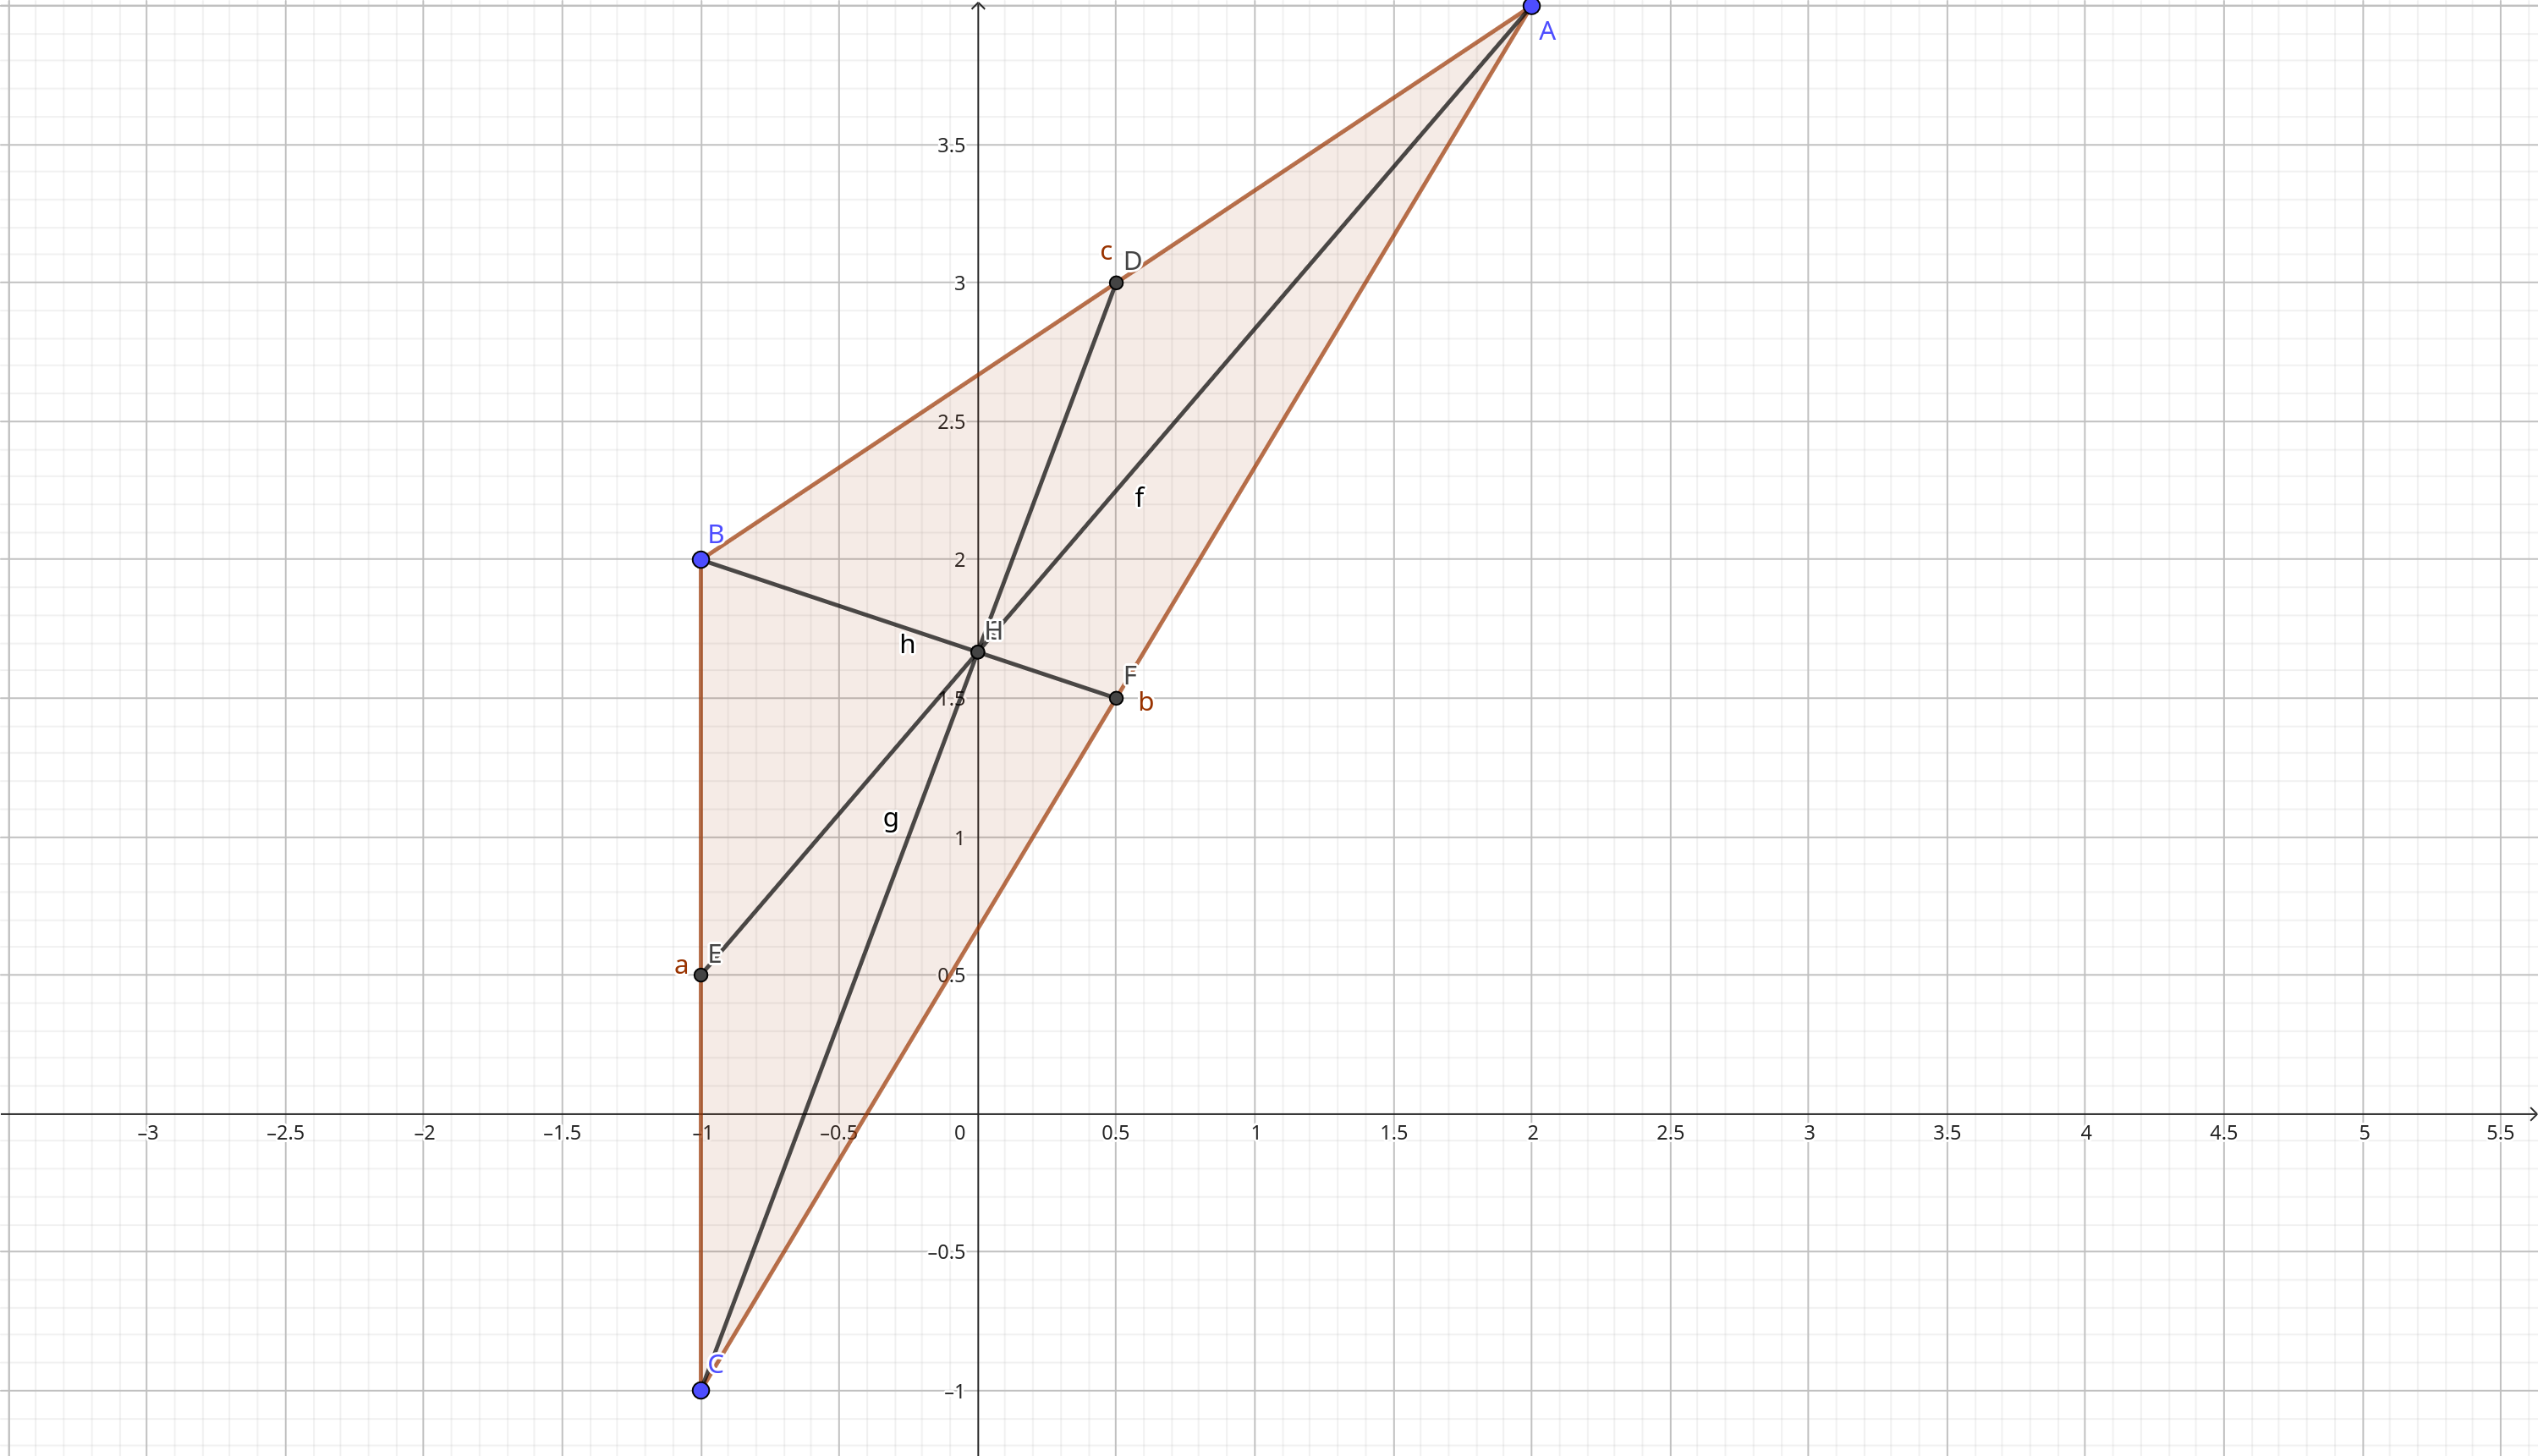
\includegraphics[height=5cm]{baricentro.png}
    \end{center}

\end{problema}
    \end{inciso}
\end{document}


    